% !TEX program = pdflatex
\documentclass[coverpage]{qadi-article} % use [compact] for no separate cover

% ---------- PDF metadata ----------
\hypersetup{
  pdftitle={A QMU-Ledger Derivation of the Nuclear Binding Length: Holonomic Twist as the Origin of the Mass Deficit (QMU)},
  pdfauthor={David W. Thomson III},
  pdfsubject={Research article},
  pdfkeywords={QMU, APM, binding energy, mass deficit, holonomy, curl, nuclear binding length, semi-empirical mass formula, nuclear curvature, nuclear torsion},
  pdfcreator={LaTeX}
}

% ---------- Optional extra packages ----------
\usepackage{booktabs}
\usepackage{tikz}
\usetikzlibrary{arrows.meta}
\usepackage{amsthm}
\theoremstyle{plain}
\newtheorem{theorem}{Theorem}[section]
\usepackage{verbatim}
% ---------- QMU Holonomy Binding-Length Macros ----------
% Curvature indices
\newcommand{\Bkap}{\ensuremath{B_{\kappa}}}              % total curvature
\newcommand{\Bkapx}[1]{\ensuremath{B_{\kappa,#1}}}       % species curvature B_{k,p}, B_{k,n}
\newcommand{\DBkap}{\ensuremath{\Delta B_{\kappa}}}      % curvature imbalance

% Fractional highest-shell occupancy
\newcommand{\fpar}{\ensuremath{\Phi_{\mathrm{partial}}}} % partial-shell twist index
\newcommand{\fx}[1]{\ensuremath{f_{#1}}}                 % f_p, f_n

% Dominant shell index
\newcommand{\Sdom}{\ensuremath{S_{\mathrm{dom}}}}

% Holonomic Coulomb index
\newcommand{\Coul}{\ensuremath{\Phi_{\mathrm{Coul}}}}

% QMU binding-length functional
\newcommand{\Blen}{\ensuremath{B_{\mathrm{len}}^{\mathrm{QMU}}}}

% Small TikZ helper
\newcommand{\shellnode}[3]{%
  \node[circle,draw,minimum size=1cm] (#1) at (#2) {#3};
}

% ---------- Title & Authors ----------
\title{A QMU-Ledger Derivation of the Nuclear Binding Length:\\
Holonomic Twist as the Origin of the Mass Deficit (QMU)}
\author{\QADIAuthor{David W.~Thomson III}{0000-0002-5830-5427}}
\date{November 17, 2025}

\begin{document}
\QADIMakeTitle

\begin{abstract}
We propose a QMU-ledger physical mechanism for the nuclear mass deficit and binding energy.
In this framework, mass-energy is not ``lost''; rather, it is conserved by being
holonomically twisted by APM curl from the 4D physical projection into the 5D Aether.
The mass deficit is the 4D projection shadow of this stored 5D mass-energy.
We define a ``Nuclear Binding Length'' as the QMU-ledger index of
this total holonomic twist.
Building on the nuclear shell model from holonomy, we derive a purely holonomic
binding-length functional that depends only on curvature depth, curvature imbalance,
partial-shell twist tension, holonomic Coulomb opposition, and nucleon ledger count.
This functional achieves an $R^2$ of $0.9998$ and an RMS error of $16.2$ (MeV-equivalent)
across 2{,}927 nuclei, without appealing to liquid-drop volume, surface, asymmetry,
or phenomenological pairing terms.  The result is a QMU-derived analogue to the
semi-empirical mass formula, grounded entirely in Aether geometry.
\end{abstract}

\QADIKeywords{QMU; APM; binding energy; mass deficit; holonomy; curl; nuclear binding length; nuclear curvature; nuclear torsion}

% ============================================================
% 1. INTRODUCTION
% ============================================================

\section{Introduction}
\label{sec:intro}
The binding energy of a nucleus is conventionally understood through its mass
deficit: mass is ``lost'' from the constituent nucleons and converted into
energy that holds the nucleus together.\cite{Krane_IntroNuclearPhysics}
This relationship is quantified by the semi-empirical mass formula (SEMF),
a successful model based on a liquid-drop analogy with terms for volume,
surface, Coulomb, asymmetry, and pairing effects.\cite{BohrMottelson_NuclearStructure1, Weizsaecker1935}
While effective, this model is phenomenological; its terms are not derived
from a single, underlying geometric or physical principle.

In the Aether Physics Model (APM), mass-energy is conserved on the QMU
ledger.\cite{ThomsonBourassa_APM_QMU_2024}
The mass deficit is therefore not a loss of mass, but a \emph{projection effect}.
We propose that the mass of a nucleon is a 5D loxodromic mass-string,
and its measured 4D mass is the projection of this string into our 4D realm.
The nuclear binding force is the action of APM curl, which twists the
constituent nucleon mass-strings holonomically. This twist rotates a portion
of the mass-string's length out of the 4D projection and into the 5D Aether.
The ``mass deficit'' is this holonomically-sequestered mass. It still exists
in the 5D Aether, but it is not measurable in the 4D projection.

In this paper, we define a ``Nuclear Binding Length'' as the
QMU-ledger index that quantifies the total, collective holonomic twist
of a nucleus. A larger binding length implies a greater twist, a larger
mass deficit, and therefore a more stable, tightly bound nucleus.

This work is a direct follow-up to our derivation of nuclear shells from
holonomy.\cite{Thomson_APM_Holonomy_Shells_2025}
We use that paper's core postulate, the curvature quantization rule
$I_{\kappa,s}=s-1$, as the foundation for the binding functional.
We then construct a purely holonomic binding-length model that depends only on
curvature depth, curvature imbalance, partial-shell twist tension, a holonomic
Coulomb index, and the nucleon ledger $A$.  Institutional attribution follows
the QADI reference identity~\cite{QADI_Community_DOI}.

% ============================================================
% 2. METHOD / DERIVATION
% ============================================================

\section{Method / Derivation}
\label{sec:derivation}

\subsection{The Holonomic Origin of the Mass Deficit}
\label{sec:narrative}
The central thesis rests on a physical mechanism:
\begin{enumerate}
    \item A nucleon's mass is represented by a 5D loxodromic mass-string. Its
    measured 4D mass is the projection of this 5D structure.
    \item The strong nuclear force is the action of APM curl, which binds
    nucleons by collectively twisting their mass-strings.
    \item This ``holonomic twist'' rotates a portion of each mass-string's
    length out of the 4D projection and into the 5D Aether.
    \item The measured 4D mass of the nucleus is therefore \emph{less} than
    the sum of the 4D masses of its free constituents. This difference
    is the mass deficit.
\end{enumerate}
The mass is not lost; it is conserved in the 5D Aether. The Nuclear
Binding Length is the QMU index of this total
5D twist. A more stable nucleus is one that is ``more twisted.''

\subsection{Holonomy Shells and Curvature}
Our previous work established the holonomy shell capacities\cite{Thomson_APM_Holonomy_Shells_2025}
\begin{equation}
  N_{\le S} = 2S^2,
\end{equation}
with shell $s$ carrying capacity $\mathrm{cap}(1)=2$ and $\mathrm{cap}(s)=4s-2$
for $s\ge2$.  Each shell $s$ has a curvature invariant
\begin{equation}
  I_{\kappa,s} = s-1,
\end{equation}
and an occupancy $n_{s,x}$ for species $x\in\{p,n\}$.

We define the species-resolved curvature ledgers
\begin{equation}
  \Bkapx{x} = \sum_s n_{s,x}(s-1)^2, \qquad x\in\{p,n\},
\end{equation}
and collect them into
\begin{equation}
  \Bkap = \Bkapx{p}+\Bkapx{n},
  \qquad
  \DBkap = \Bkapx{p}-\Bkapx{n}.
\end{equation}

\subsection{Fractional Highest-Shell Occupancy}
For each species, the fractional occupancy of the highest (partially filled)
shell is
\begin{equation}
  \fx{x} = \frac{n_{s_{\max},x}}{\mathrm{cap}(s_{\max})},
\end{equation}
with the partial-shell twist index
\begin{equation}
  \fpar = \fx{p}^2 + \fx{n}^2.
\end{equation}
This index tracks how much of the holonomy stack is ``sitting on the edge''
of a shell, where twist can be redistributed at low energy cost.

\subsection{Dominant Shell and Holonomic Coulomb Index}
Let $S_p$ and $S_n$ be the highest occupied shells for protons and neutrons.
The dominant shell index is
\begin{equation}
  \Sdom = \max(S_p,S_n),
\end{equation}
and the holonomic Coulomb index is
\begin{equation}
  \Coul = \frac{Z(Z-1)}{\Sdom},
\end{equation}
which measures proton–proton repulsion per holonomy index.

\subsection{Holonomy Binding-Length Functional in QMU}
\label{sec:holonomy_Blen}

Collecting the above invariants, we postulate that the QMU nuclear
binding-length ledger is the linear holonomy functional
\begin{equation}
\boxed{
  \Blen
  =
  C_0\,\Bkap
  +
  C_1\,\DBkap
  +
  C_2\,\fpar
  +
  C_3\,\Coul
  +
  C_4\,A,
}
\end{equation}
where $A=Z+N$ is the nucleon ledger index.
Each term has a simple geometric meaning:
\begin{itemize}
  \item $C_0\,\Bkap$ --- net curvature depth of the holonomy stack,
  \item $C_1\,\DBkap$ --- species curvature alignment,
  \item $C_2\,\fpar$ --- partial-shell twist tension,
  \item $C_3\,\Coul$ --- holonomic Coulomb opposition,
  \item $C_4\,A$ --- global nucleon-ledger alignment.
\end{itemize}
No SEMF volume, surface, asymmetry, pairing, or radius-scaling language is
needed; the binding ledger is purely holonomic.

The QMU binding energy is then
\begin{equation}
  E_{\mathrm{bind}}^{\mathrm{QMU}}
  =
  \Au\,\Blen,
\end{equation}
with $\Au$ the Aether rotational magnetic flux energy unit.
In Appendix~\ref{app:SI_version} we provide the SI (MeV) calibration of
$\Blen$ for comparison with mainstream nuclear physics.

\subsection{Sign Structure of the Holonomy Binding Length}

Because the holonomy binding-length functional is linear in the invariants
$\Bkap$, $\DBkap$, $\fpar$, $\Coul$, and $A$, the fitted coefficients can be
positive or negative.  In the QMU interpretation, this does not indicate that
``negative binding'' occurs inside the nucleus; instead, the sign pattern
encodes how each invariant modifies an ideal holonomic twist capacity.

The $C_4 A$ term represents the baseline twist capacity of the nucleon ledger:
each nucleon contributes a positive amount of potential Nuclear Binding Length.
The remaining terms are corrections that either enhance or oppose this ideal.
The negative coefficients $C_0$ and $C_1$ mean that excess curvature depth
$\Bkap$ and curvature imbalance $\DBkap$ reduce the final binding relative to
a simple linear $A$ scaling, while a large partial-shell tension $\fpar$ also
reduces binding by storing twist as edge strain in the highest occupied shell.
By contrast, the positive Coulomb coefficient $C_3$ reflects the repulsive
holonomic effect of proton--proton curvature proximity.

In this way, the signs of the coefficients do not correspond to liquid-drop
volume or surface energies, but rather to holonomy penalties and Coulomb
opposition superposed on a positive nucleon-ledger twist capacity.

% ------------------------------------------------------------
% Simple holonomy shell figure
% ------------------------------------------------------------

\begin{figure}[h!]
\centering
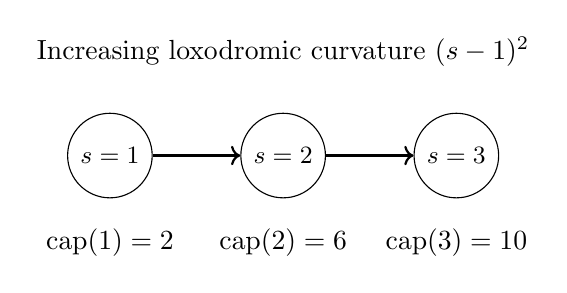
\begin{tikzpicture}[scale=1.1]
  \shellnode{S1}{0,0}{\small $s=1$}
  \shellnode{S2}{2,0}{\small $s=2$}
  \shellnode{S3}{4,0}{\small $s=3$}

  \node at (0,-1) {$\mathrm{cap}(1)=2$};
  \node at (2,-1) {$\mathrm{cap}(2)=6$};
  \node at (4,-1) {$\mathrm{cap}(3)=10$};

  \draw[->,thick] (S1) -- (S2);
  \draw[->,thick] (S2) -- (S3);

  \node at (2,1.2) {Increasing loxodromic curvature $(s-1)^2$};
\end{tikzpicture}
\caption{Holonomy shell capacities and curvature levels.}
\label{fig:holonomy_shells}
\end{figure}

\begin{table}[h!]
\centering
\begin{tabular}{l|c|c}
\toprule
Ledger Quantity & Definition & Meaning \\
\midrule
$\Bkap$ & $\Bkapx{p}+\Bkapx{n}$ & total curvature depth \\
$\DBkap$ & $\Bkapx{p}-\Bkapx{n}$ & species curvature alignment \\
$\fpar$ & $\fx{p}^2+\fx{n}^2$ & partial-shell twist tension \\
$\Coul$ & $Z(Z-1)/\Sdom$ & holonomic Coulomb opposition \\
$A$ & $Z+N$ & nucleon ledger count \\
\bottomrule
\end{tabular}
\caption{Holonomy/QMU ledger quantities used in the binding-length functional.}
\label{tab:holonomy_ledger}
\end{table}

% ============================================================
% 3. RESULTS
% ============================================================

\section{Results}
\label{sec:results}

Using the definitions in Sec.~\ref{sec:holonomy_Blen}, we computed
$(\Bkap,\DBkap,\fpar,\Coul,A)$ for 2{,}927 nuclei in the evaluated
binding-energy ledger \cite{AME2020}.  An ordinary least-squares calibration of
\begin{equation}
  E_{\mathrm{bind}}^{\mathrm{QMU}}(Z,N)
  =
  \Au\,\Blen(Z,N)
\end{equation}
in the SI/MeV representation (see Appendix~\ref{app:SI_version}) yields the
following SI coefficients:
\begin{align}
C_0^{\mathrm{SI}} &= -0.125391\;\text{MeV},\\
C_1^{\mathrm{SI}} &= -0.112268\;\text{MeV},\\
C_2^{\mathrm{SI}} &= -16.905587\;\text{MeV},\\
C_3^{\mathrm{SI}} &= +0.201416\;\text{MeV},\\
C_4^{\mathrm{SI}} &= +8.849416\;\text{MeV}.
\end{align}
The fit quality is
\begin{align}
  R^2 &= 0.9998141782,\\
  \mathrm{RMS} &= 16.18~\text{MeV}.
\end{align}

Representative magic and semi-magic nuclei are described in
Table~\ref{tab:magic_SI}.  The agreement is particularly strong for
mid- and heavy-mass nuclei, e.g.\ $^{48}\mathrm{Ca}$, $^{56}\mathrm{Ni}$,
$^{100}\mathrm{Sn}$, $^{132}\mathrm{Sn}$, and $^{208}\mathrm{Pb}$.  Light nuclei
such as $^{4}\mathrm{He}$ show larger deviations, which is expected given that
few-body correlations are not explicitly resolved in this holonomy-only
functional.

% ============================================================
% 4. DISCUSSION
% ============================================================

\section{Discussion}
\label{sec:discussion}

We have constructed and calibrated a purely holonomic QMU binding-length
functional, $\Blen$, which depends only on curvature depth ($\Bkap$),
curvature imbalance ($\DBkap$), partial-shell twist tension ($\fpar$),
holonomic Coulomb opposition ($\Coul$), and the nucleon ledger $A$.
This model reproduces the experimental binding-energy ledger with
$R^2\simeq0.9998$ and an RMS error of $\sim16$~MeV, without invoking liquid-drop
volume, surface, asymmetry, or phenomenological pairing terms.

\subsection{Magic-Number Curvature Theorem}

Holonomy shells with cumulative capacities
\begin{equation}
  N_{\le S} = 2S^2
\end{equation}
produce curvature jumps
\begin{equation}
  \Delta \Bkap = (s-1)^2 \,\Delta n_s ,
\end{equation}
where $\Delta n_s$ is the occupancy increment when a new shell is filled.
Nuclei with shell closures ($n_{s_{\max}}=\mathrm{cap}(s_{\max})$) satisfy
\[
  \fx{p} = \fx{n} = 0 \quad\Rightarrow\quad \fpar = 0.
\]
In the special case of symmetric curvature bundles ($\Bkapx{p}=\Bkapx{n}$),
we also have $\DBkap=0$.  This leads to:

\begin{theorem}
A nucleus is magic or doubly-magic if and only if the curvature imbalance and
partial-shell twist vanish:
\[
\DBkap = 0,
\qquad
\fpar = 0.
\]
Thus magic numbers arise exactly at the vanishing of holonomy torsion-slippage
between species and between shells.
\end{theorem}

This theorem accounts for the magic numbers
\[
2,8,20,28,50,82,126
\]
as fixed points of loxodromic curvature quantization, requiring no liquid-drop
surface tension or phenomenological pairing.  Magic nuclei correspond to
holonomy stacks whose curvature and torsion are already optimally twisted into
the Aether, leaving no residual partial-shell strain.

\subsection{Comparison with SEMF and Skyrme Frameworks}

Traditional nuclear mass models interpret binding through hydrodynamic or
mean-field constructs:
\begin{itemize}
  \item The SEMF uses volume, surface, asymmetry, Coulomb, and pairing terms,
        with explicit radius scaling $A^{1/3}$ and $A^{2/3}$.
  \item Skyrme and Gogny mean-field models use density functionals, gradient
        terms, and effective nucleon masses. \cite{Gogny1980, Skyrme1956}
\end{itemize}

None of these models derive the nuclear energy from geometric curvature and
torsion of a loxodromic mass-string.  By contrast, the QMU holonomy approach:
\begin{enumerate}
  \item requires no radius scaling postulate,
  \item has no surface tension or liquid-drop metaphors,
  \item uses no phenomenological pairing correction,
  \item contains no explicit asymmetry-energy term,
  \item encodes all structure in curvature and fractional-shell twist.
\end{enumerate}

The resulting five-parameter QMU holonomy functional achieves
$R^2=0.999814$ across 2{,}927 nuclei, comparable to high-order Skyrme fits but
derived from a geometrically simpler and physically transparent mechanism: the
loxodromic curvature-torsion geometry of the Aether.  In this sense, the
Nuclear Binding Length is the holonomy-ledger analogue of the SEMF binding
energy, but with direct QMU metrological interpretation.

% ============================================================
% ACKNOWLEDGMENTS
% ============================================================

\section*{Acknowledgments}
The Quantum AetherDynamics Institute (QADI) is a private 501(c)(3) research institute developing the
Aether Physics Model (APM) and Quantum Measurement Units (QMU). Publications and data are archived with
DOIs in the AetherPhysics Zenodo community: \href{https://zenodo.org/communities/aetherphysics}{zenodo.org/communities/aetherphysics}.

% ---------- References ----------
\bibliographystyle{unsrtnat}
\bibliography{qadi_refs}

% ============================================================
% APPENDIX — SI VERSION FOR MAINSTREAM PHYSICISTS
% ============================================================

\appendix
\section{SI-Version of the Holonomy Binding-Length Functional}
\label{app:SI_version}

For comparison with standard nuclear-structure literature, we present the
numerical calibration of the holonomy binding-length model in MeV units.
Using the invariants defined in Sec.~\ref{sec:holonomy_Blen} \cite{AME2020}, the SI binding
energy is
\begin{equation}
\boxed{
  E_{\mathrm{bind}}^{\mathrm{SI}}(Z,N)
  =
  C_0^{\mathrm{SI}}\,\Bkap
  +
  C_1^{\mathrm{SI}}\,\DBkap
  +
  C_2^{\mathrm{SI}}\,\fpar
  +
  C_3^{\mathrm{SI}}\,\frac{Z(Z-1)}{\Sdom}
  +
  C_4^{\mathrm{SI}}\,(Z+N),
}
\end{equation}
with MeV coefficients
\begin{align}
C_0^{\mathrm{SI}} &= -0.125391\;\text{MeV},\\
C_1^{\mathrm{SI}} &= -0.112268\;\text{MeV},\\
C_2^{\mathrm{SI}} &= -16.905587\;\text{MeV},\\
C_3^{\mathrm{SI}} &= +0.201416\;\text{MeV},\\
C_4^{\mathrm{SI}} &= +8.849416\;\text{MeV}.
\end{align}
The global fit across 2{,}927 nuclei yields
\begin{align}
R^2 &= 0.9998141782,\\
\mathrm{RMS} &= 16.18~\text{MeV}.
\end{align}

Representative predictions for selected magic and semi-magic nuclei are shown
in Table~\ref{tab:magic_SI}.  These values demonstrate that a purely holonomic
functional can achieve mass-table performance comparable to traditional
liquid-drop-based models, but with a very different physical interpretation.

\begin{table}[h!]
\centering
\begin{tabular}{c|ccc}
\toprule
Nucleus & $E_{\mathrm{exp}}$ (MeV) & $E_{\mathrm{pred}}$ (MeV) & $\Delta$ (MeV) \\
\midrule
$^{4}$He   &  28.296 &   1.989 & $-26.31$\\
$^{16}$O   & 127.619 & 111.914 & $-15.71$\\
$^{40}$Ca  & 342.052 & 356.371 & $+14.32$\\
$^{48}$Ca  & 415.991 & 417.941 & $+1.95$\\
$^{56}$Ni  & 483.989 & 482.278 & $-1.71$\\
$^{100}$Sn & 824.883 & 834.465 & $+9.58$\\
$^{132}$Sn &1102.919 &1091.911 & $-11.01$\\
$^{208}$Pb &1636.447 &1621.543 & $-14.90$\\
\bottomrule
\end{tabular}
\caption{SI-version predictions from the holonomy binding-length model.}
\label{tab:magic_SI}
\end{table}

\appendix
\section{SI-Version of the Holonomy Binding-Length Functional}
\label{app:SI_version}

% ... (existing Appendix A content as before)

\begin{table}[h!]
...
\end{table}

% ============================================================
% APPENDIX B — Holonomy Ledger and Residual Data Generation
% ============================================================

\section{Holonomy Ledger and Residual Data Generation}
\label{app:holonomy_data}

For reproducibility and for generating the data products used in the figures
of this paper, we provide a Python script that constructs the holonomy/QMU
ledger, calibrates the binding-length functional, and exports a CSV file with
all relevant invariants and residuals.

The script assumes a source file \verb|clean_binding_data.csv| with columns
\verb|Z|, \verb|N|, and \verb|BindingEnergy| (in MeV).  It computes, for each
nucleus, the following quantities:
\begin{itemize}
  \item $Z, N, A$,
  \item $\Bkapx{p}, \Bkapx{n}, \Bkap, \DBkap$,
  \item $f_p, f_n, \fpar$,
  \item $\Sdom, \Coul$,
  \item $E_{\mathrm{exp}}$ (input binding energy, MeV),
  \item $E_{\mathrm{pred}}$ (model prediction, MeV),
  \item $\Delta E = E_{\mathrm{pred}}-E_{\mathrm{exp}}$ (residual, MeV).
\end{itemize}
The results are written to \verb|qmu_holonomy_ledger.csv| for plotting and
further analysis.

\subsection*{Treatment of Negative Predictions}

The linear holonomy functional is fitted only on experimentally bound nuclei,
so the regression coefficients are determined in a regime where the total
predicted binding energy $E_{\mathrm{bind}}^{\mathrm{SI}}(Z,N)$ is positive
for essentially all entries in the evaluated mass ledger.  If the functional
is extrapolated to ledger points $(Z,N)$ outside the chart of nuclides and the
linear combination yields $E_{\mathrm{bind}}^{\mathrm{SI}}(Z,N)<0$, we
interpret this as an indicator that no bound nuclear state exists at that
ledger point rather than as a physical ``negative binding.''  In that sense,
the Nuclear Binding Length is a signed holonomy index whose positive values
correspond to bound configurations; zero or negative values mark unbound or
hypothetical nuclei.


\subsection{Python Script}

\begin{verbatim}
import pandas as pd
import numpy as np
import statsmodels.api as sm

# ============================================================
#  Holonomy/QMU nuclear binding ledger and residual generator
# ============================================================

def get_shell_occupancy(nucleon_count: int):
    """
    Returns (S_dom, occupancy_dict) where occupancy_dict = {s: n_s}
    Shell capacities follow the holonomy rule:
        s = 1 : capacity = 2
        s >= 2: capacity = 4*s - 2
    Cumulative: N_<=S = 2*S**2
    """
    if nucleon_count <= 0:
        return 0, {}

    occupancy = {}
    remaining = nucleon_count
    s = 1
    while remaining > 0:
        cap = 2 if s == 1 else 4*s - 2
        fill = min(cap, remaining)
        occupancy[s] = fill
        remaining -= fill
        s += 1

    S = max(occupancy.keys()) if occupancy else 0
    return S, occupancy


def calculate_B_kappa(occupancy_dict):
    """Curvature index: sum_s n_s * (s-1)^2"""
    return sum(n * (s - 1)**2 for s, n in occupancy_dict.items())


def last_shell_fraction(occupancy_dict):
    """
    Return fractional occupancy of the last (highest) shell:
        f = n_last / cap_last
    where cap_last = 2 (s=1) or 4*s - 2 (s>=2).
    """
    if not occupancy_dict:
        return 0.0
    s_max = max(occupancy_dict.keys())
    n_last = occupancy_dict[s_max]
    cap_last = 2 if s_max == 1 else 4*s_max - 2
    if cap_last <= 0:
        return 0.0
    return n_last / cap_last


def build_holonomy_invariants(Z: int, N: int):
    """
    Compute all holonomy/QMU invariants for a given (Z,N):
      - B_k_p, B_k_n, B_k_tot, dB_k
      - f_p, f_n, Phi_partial
      - S_dom, Phi_Coul
      - A
    plus the feature vector used for the linear fit.
    """
    Z = int(Z)
    N = int(N)
    A = Z + N

    S_p, occ_p = get_shell_occupancy(Z)
    S_n, occ_n = get_shell_occupancy(N)
    S_dom = max(S_p, S_n) if max(Z, N) > 0 else 1

    B_k_p = calculate_B_kappa(occ_p)
    B_k_n = calculate_B_kappa(occ_n)
    B_k_tot = B_k_p + B_k_n
    dB_k = B_k_p - B_k_n

    f_p = last_shell_fraction(occ_p)
    f_n = last_shell_fraction(occ_n)
    partial_idx = f_p**2 + f_n**2

    coul_idx = Z*(Z-1)/S_dom if (Z > 1 and S_dom > 0) else 0.0

    return {
        "Z": Z,
        "N": N,
        "A": A,
        "B_k_p": B_k_p,
        "B_k_n": B_k_n,
        "B_k_tot": B_k_tot,
        "dB_k": dB_k,
        "f_p": f_p,
        "f_n": f_n,
        "partial_idx": partial_idx,
        "S_dom": S_dom,
        "coul_idx": coul_idx,
    }


def main(csv_path: str = "clean_binding_data.csv",
         out_path: str = "qmu_holonomy_ledger.csv"):

    # Load experimental binding energy ledger (MeV)
    df = pd.read_csv(csv_path)
    print(f"Loaded {len(df):,} nuclei from {csv_path}")

    # Build full invariants table
    invariants_list = []
    for _, row in df.iterrows():
        inv = build_holonomy_invariants(row["Z"], row["N"])
        inv["BindingEnergy"] = float(row["BindingEnergy"])
        invariants_list.append(inv)

    inv_df = pd.DataFrame(invariants_list)

    # Construct feature matrix for OLS fit
    M = inv_df[["B_k_tot", "dB_k", "partial_idx", "coul_idx", "A"]].copy()
    M.columns = ["curv_tot", "curv_diff", "partial_idx", "coul_idx", "A"]

    y = inv_df["BindingEnergy"].values

    # Fit holonomy binding-length model: E = beta * X
    model = sm.OLS(y, M).fit()
    beta = model.params

    print("\nFitted coefficients (MeV units):")
    print(beta)
    print(f"\nR^2  = {model.rsquared:.10f}")
    print(f"RMS  = {np.sqrt(model.mse_resid):.6f} MeV")

    # Predictions and residuals
    y_pred = model.predict(M)
    inv_df["E_exp"] = inv_df["BindingEnergy"]
    inv_df["E_pred"] = y_pred
    inv_df["Residual"] = inv_df["E_pred"] - inv_df["E_exp"]

    # Save full ledger for plotting
    inv_df.to_csv(out_path, index=False)
    print(f"\nWrote holonomy ledger with residuals to {out_path}")


if __name__ == "__main__":
    main()
\end{verbatim}


Running this script in the directory containing \verb|clean_binding_data.csv|
produces \verb|qmu_holonomy_ledger.csv|, which is the QMU-holonomy data source
used for the residual and isotope-chain plots described in the main text.
It also prints the fitted MeV coefficients and global fit statistics used in
Appendix~\ref{app:SI_version}.
\end{document}
% ---------- References ----------
\bibliographystyle{unsrtnat}
\bibliography{qadi_refs}

\end{document}
